\documentclass[conference]{IEEEtran}
\IEEEoverridecommandlockouts

\usepackage{amssymb}
\usepackage[table]{xcolor}
\usepackage{xspace}
\usepackage{booktabs}
\usepackage{amsmath}
\usepackage{graphicx}
\usepackage{algorithm}
\usepackage{algpseudocode}
\usepackage{float}
\usepackage{cite}
\usepackage{subcaption}
\usepackage{makecell}
\usepackage{xurl}
\usepackage{tikz}
\usetikzlibrary{arrows.meta, positioning, fit, calc}

% ---- Macros ----
\newcommand{\smarm}{SMARM\xspace}
\newcommand{\tdis}{$t_{\mathrm{disabled}}$\xspace}
\newcommand{\FAR}{FAR\xspace}
\newcommand{\smarmcopy}{SMARM+Copy\xspace}
\newcommand{\smarmlock}{SMARM+Lock\xspace}

\newcommand\oak[1]{\textcolor{red}{OAK: #1}}

\begin{document}

\title{Towards Fully Interruptible Shuffled Measurement for Remote Attestation}

% DOUBLE-BLIND: comment out \author before submitting if required
\author{
  \IEEEauthorblockN{Amarin Laohajirapan, Norrathep Rattanavipanon}
  \IEEEauthorblockA{College of Computing,
    Prince of Songkla University, Phuket Campus, Thailand \\
    norrathep.r@psu.ac.th}
}

\maketitle

% ================================================================
\begin{abstract}
Remote attestation (RA) detects software compromise on IoT devices, but
classical RA keeps interrupts disabled for a full memory scan and can
block real-time work for hundreds of milliseconds.
SMARM instead measures memory in a secret shuffled order so attestation
can be interrupted between blocks while still resisting
\emph{roving malware}.
The original design was evaluated on a formally verified microkernel
stack, not on widely used production RTOSes.
We port SMARM to FreeRTOS on ARM TrustZone-M and show that, although
interrupts are re-enabled between blocks, hashing each block with
interrupts disabled still breaks common real-time periods when the block
size grows on commodity Cortex-M33 hardware.
We study two TrustZone-M enhancements that keep the block snapshot
atomic while allowing hash work to coexist with interrupts.
\emph{Atomic Copy} disables interrupts only around a short memory copy
into Secure RAM, then hashes with interrupts enabled.
\emph{SAU remapping} instead punches a temporary hole in Non-Secure SAU
coverage so the target block is Secure by default during the hash, with
no copy buffer. Both restore Frequency Accuracy Ratio
(FAR)~$\approx 1.0$ for all tested block sizes up to $B{=}4096$~bytes
and workloads from $10$ to $1000$~Hz on STM32L552ZE with FreeRTOS.
\end{abstract}

\begin{IEEEkeywords}
Remote attestation, IoT security, TrustZone-M, SAU, RTOS, SMARM,
interrupt latency
\end{IEEEkeywords}

% ================================================================
\section{Introduction}
\label{sec:intro}

Modern societies increasingly depend on Internet-of-Things (IoT) devices across domains ranging from smart factories, where industrial sensors support monitoring and automation, to smart homes, where devices such as smart lights and robotic vacuum cleaners improve convenience. 
Since many IoT devices are designed to be inexpensive and energy-efficient, they typically operate on resource-constrained microcontrollers (MCUs) with limited RAM, flash storage, and energy budgets. These constraints often preclude sophisticated monolithic operating systems and the malware defenses available on higher-end devices.

Remote attestation (RA)~\cite{eldefrawy2012smart,nunes2019vrased,eldefrawy2017hydra} has emerged as an inexpensive technique for detecting malware compromise on resource-constrained IoT devices. In RA, an IoT device, called the \emph{prover}, executes a measurement routines that hashes its software image (i.e., the code stored in flash memory) and returns the measurement result in an authenticated response (e.g., using a message authentication code (MAC) or digital signature). 
An external trusted party, called the \emph{verifier}, compares this measurement against that of the expected software image to determine whether the prover's software has been modified and hence be able to deduce whether a malware compromise happens on the prover.

Traditional RA requires the measurement routine to execute atomically with interrupts disabled. This atomic execution is necessary to prevent \emph{roving malware} from evading detection by relocating itself to a region that has already been measured. On low-end MCUs, however, the resulting non-preemptible interval can exceed $450$~ms~\cite{nunes2019vrased}. Such prolonged interrupt disablement can severely interfere with real-time applications whose correctness depends on completing time-critical tasks within their deadlines.

To relax the atomicity requirement, SMARM~\cite{carpent2018smarm} introduces a new technique, called \emph{shuffled measurement}, which permits interrupts between the measurements of individual memory blocks. To defend against roving malware, SMARM measures the blocks comprising the software image in a random and secret order. Because malware does not know which blocks have already been measured, it cannot reliably relocate itself to an inspected block to evade detection. Although this approach does not provide the deterministic protection of fully atomic measurement, it makes evasion probabilistically difficult while reducing the non-preemptible interval from the measurement of the entire software image to that of a single block.

Despite this improvement, SMARM's maximum non-preemptible interval remains determined by its block size. Prior work~\cite{} shows that using larger blocks can reduce the total attestation time by lowering per-block processing overhead. However, a larger block also takes longer to measure, thereby extending each non-preemptible interval and potentially delaying time-critical tasks beyond their deadlines. Conversely, smaller blocks shorten these intervals but increase the number of blocks and the associated computational overhead, resulting in longer attestation times and greater energy consumption. SMARM therefore exposes an inherent tradeoff between real-time responsiveness and energy efficiency, which is particularly problematic for battery-powered IoT devices.

Motivated by this observation, we propose two independent enhancements to shuffled measurement that further shorten its non-interruptible periods, allowing the technique to coexist with a broader range of time-sensitive applications. 
Our contributions are as follows:

\begin{itemize}
\item We propose \smarmcopy, which reduces each non-interruptible period from the time required to hash one memory block to the substantially shorter time required to copy that block.

\item Since \smarmcopy's non-interruptible period remains proportional to the block size, we further propose \smarmlock, another enhancement that makes this interval effectively independent of block size. 
\smarmlock reduces interrupt disablement to a negligible, constant-duration operation, at the cost of introducing a probability of interference with concurrent application memory accesses.

\item We implement \smarmcopy and \smarmlock on Nucleo-...~\cite{} a low-end MCU-equipped development board with a TrustZone-M--based trusted execution environment and evaluate them on real hardware. Our results demonstrate that both mechanisms substantially reduce SMARM's non-interruptible periods, thereby improving its compatibility with time-sensitive embedded applications.

\end{itemize}


% threat with a different
% contract: memory is measured in a one-time secret shuffled order derived
% from the verifier challenge and a protected key, interrupts are allowed
% \emph{between} blocks, and malware that does not know the remaining
% order cannot reliably hide. The original SMARM design and analysis were
% grounded in a SMART/HYDRA-style trust anchor on a formally verified
% microkernel (seL4)~\cite{eldefrawy2017hydra,carpent2018smarm}. To our
% knowledge it had not been ported to widely deployed production RTOSes
% such as FreeRTOS or Zephyr. We therefore first port SMARM to FreeRTOS
% on ARM TrustZone-M and evaluate real-time coexistence with a Frequency
% Accuracy Ratio (\FAR) metric. The port shows that SMARM still fails to
% keep $\mathrm{FAR}\approx 1.0$ for $B\geq 2048$~bytes at a $1000$~Hz
% workload, because each block's SHA-256 update remains fully
% non-interruptible---even though the scan as a whole is interruptible
% between blocks.

% This paper makes two contributions that address that remaining
% bottleneck without changing SMARM's shuffled-measurement structure
% against roving malware:

% \begin{enumerate}
%   \item \textbf{Atomic Copy.} We keep interrupts disabled only while
%     copying the chosen block into a Secure-world buffer, then run
%     HMAC-SHA256 with interrupts enabled. On Cortex-M33 this cuts
%     \tdis by about $15\times$ versus hashing under interrupt disable,
%     and restores $\mathrm{FAR}\approx 1.0$ for all evaluated block sizes.
%   \item \textbf{SAU remapping.} We temporarily leave a hole in the
%     Non-Secure SAU coverage of a dedicated data window so the selected
%     block becomes Secure by default~\cite{armv8m-arm,an5347}, hash it
%     in place, then restore Non-Secure coverage. This removes the copy
%     buffer while keeping interrupts enabled during hashing, and restores
%     $\mathrm{FAR}\approx 1.0$ across all evaluated workloads.
% \end{enumerate}

% A longer journal version covers multi-RTOS ports (including Zephyr),
% storage-reduction variants (PRF/FPE), and energy measurements. Here we
% focus on the FreeRTOS/TrustZone-M bottleneck and the two mitigations
% above.

% ================================================================
\section{Background}
\label{sec:background}

\subsection{RA Atomicity and SMARM}

\oak{Briefly mention RA workflow, i.e., challenge-response between prover and verifier etc.}
Classical RA often disables interrupts for the whole measurement so that
\emph{roving malware} cannot move itself while memory is being
hashed~\cite{eldefrawy2012smart,nunes2019vrased}.
SMARM~\cite{carpent2018smarm} instead derives a one-time permutation
$\sigma$ from the verifier challenge and a secret key $k$, then measures
blocks $M_{\sigma(i)}$ one by one, re-enabling interrupts between
blocks. The security claim is not ``malware cannot interrupt''; it is
that malware without knowledge of the remaining secret order cannot
reliably relocate to escape detection, and repeated independent sessions
drive the escape probability down~\cite{carpent2018smarm}.
SMARM requires three security properties:
\begin{enumerate}
  \item \textbf{(S1) Controlled Execution.}
    The attestation service is reachable only through defined
    entry/exit points (on our platform, NSC gates into Secure
    world). Interrupts may be re-enabled only
    \emph{between} block measurements---never in the middle of a
    protected capture step---so malware cannot splice itself into a
    half-measured block.
  \item \textbf{(S2) Key Secrecy.}
    The attestation key $k$ is stored in memory inaccessible to
    untrusted Non-Secure software, so malware cannot forge a valid
    report.
  \item \textbf{(S3) Private Measurement Order.}
    The permutation $\sigma$ is stored in memory inaccessible to
    KFV (known-future-visit) malware, so the adversary cannot
    predict which remaining blocks will be measured next and relocate
    ahead of the scan.
\end{enumerate}
The original SMARM evaluation used a HYDRA/seL4 trust
anchor~\cite{eldefrawy2017hydra,carpent2018smarm}. Our FreeRTOS port
keeps the same shuffled protocol and uses SMARM (interruptible between
blocks, but hash still IRQ-off per block) as the experimental baseline
against which Atomic Copy and SAU remapping are compared.

\subsection{TrustZone-M Platform}

\oak{Mention TZ-M background, i.e., S vs NS Worlds and SAU. Nucleo board is not a background; its an experiment setup.}
We implement SMARM on the STM32L552ZE Nucleo-144 board (Cortex-M33 at
$110$~MHz) using TrustZone-M as the trust
anchor~\cite{trustzone2025,an5347}. Untrusted FreeRTOS tasks run
Non-Secure; the attestation service, key $k$, and permutation $\sigma$
reside in Secure RAM and are reachable only through Non-Secure Callable
(NSC) entries (Fig.~\ref{fig:system_model}). Between blocks, the RTOS can
preempt the Non-Secure wrapper task and run a high-priority real-time
task (Fig.~\ref{fig:workflow}).
\oak{cite to-be-posted arxiv paper. We shouldnt claim that we do this.}

\begin{figure}[!t]
  \centering
  \includegraphics[width=0.92\linewidth]{system-threat-model.pdf}
  \caption{SMARM on FreeRTOS with TrustZone-M. The Non-Secure wrapper
    calls a Secure service through NSC. Key $k$ and permutation
    $\sigma$ stay in Secure RAM.}
  \label{fig:system_model}
\end{figure}

\begin{figure}[!t]
  \centering
  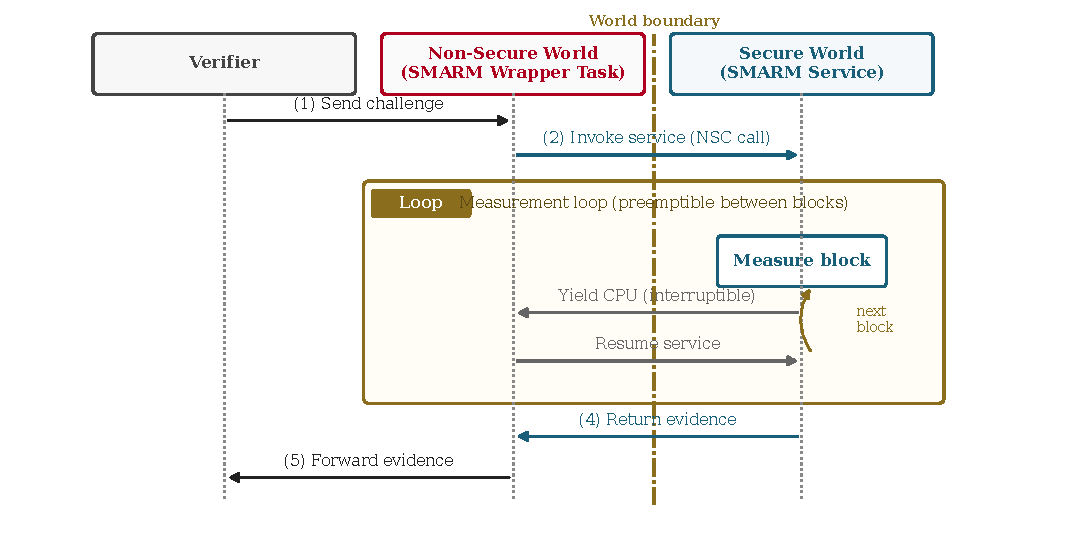
\includegraphics[width=0.92\linewidth]{smarm_workflow.pdf}
  \caption{End-to-end SMARM workflow. Real-time tasks may run between
    consecutive block measurements.}
  \label{fig:workflow}
\end{figure}

\subsection{FAR Metric}

We report real-time availability as
\[
  \mathrm{FAR}=\frac{f_{\mathrm{observed}}}{f_{\mathrm{baseline}}},
\]
where $f_{\mathrm{observed}}$ is the real-time task frequency during
attestation and $f_{\mathrm{baseline}}$ is the frequency without
attestation \oak{is this what we defined for FAR? Isn't baseline defined for attestation with interrupts enabled?}. Values near $1.0$ mean little interference.

Table~\ref{tab:ra_comparison} places traditional RA, SMARM, and our two
enhancements side by side.

\begin{table}[!t]
  \centering
  \caption{Comparison of attestation approaches for real-time IoT devices.}
  \label{tab:ra_comparison}
  \renewcommand{\arraystretch}{1.1}
  \small
  \setlength{\tabcolsep}{2.5pt}
  \begin{tabular}{lcccc}
    \toprule
    \textbf{Approach} &
    \textbf{RT-safe} &
    \makecell{\textbf{Extra} \\ \textbf{RAM}} &
    \makecell{\textbf{Atomic} \\ \textbf{window}} &
    \textbf{RTOS} \\
    \midrule
    Traditional RA~\cite{eldefrawy2012smart} &
      \texttimes & 0 & Full scan & \texttimes \\
    SMARM~\cite{carpent2018smarm} &
      Partial & 0 & Per-block hash & \texttimes \\
    \textbf{Atomic Copy} &
      \checkmark & $+B$ & Per-block copy & \checkmark \\
    \textbf{SAU remapping} &
      \checkmark & 0 & Secure hole, IRQ on & \checkmark \\
    \bottomrule
  \end{tabular}
\end{table}

% ================================================================
\section{Motivation}
\label{sec:motivation}

In baseline SMARM, each block update disables interrupts for the full
SHA-256 work on that block. With about $1.1$~MB/s hash throughput on our
board, \tdis grows from $0.062$~ms at $B{=}64$~bytes to $3.75$~ms at
$B{=}4096$~bytes. A $1000$~Hz task has a $1$~ms period, so large blocks
hold the CPU through several missed activations.

Figure~\ref{fig:timing_diagram} sketches the interrupt-disabled windows
for traditional RA, SMARM baseline, and Atomic Copy. Figure~\ref{fig:setup_and_baseline_far}
shows the measured impact: under a $1000$~Hz workload,
$\mathrm{FAR}$ stays near $1.0$ only for $B\leq 1024$~bytes and falls
sharply at $B\geq 2048$~bytes (down to about $0.27$ at $B{=}4096$).

\begin{figure}[!t]
  \centering
  \includegraphics[width=\linewidth]{timing_diagram.png}
  \caption{Interrupt-disabled windows. Traditional RA covers the full
    scan. SMARM limits disability to one block hash. Atomic Copy further
    limits it to one block copy.}
  \label{fig:timing_diagram}
\end{figure}

\begin{figure}[!t]
  \centering
  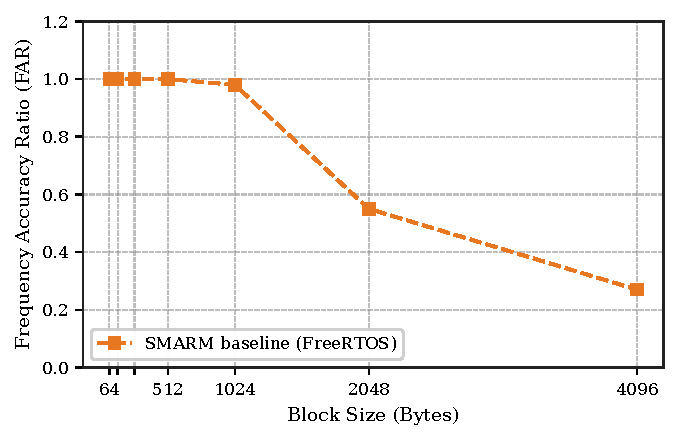
\includegraphics[width=\linewidth]{far_1000.pdf}
  \caption{FAR of baseline SMARM under a $1000$~Hz real-time workload
    across block sizes (FreeRTOS/Zephyr). Values stay near $1.0$ for
    $B\leq 1024$~bytes and drop for larger $B$.}
  \label{fig:setup_and_baseline_far}
\end{figure}

\textbf{Root cause.} Cryptographic hashing itself does not need to be
atomic. What must be atomic is the capture of the block bytes that feed
the hash. The next section presents two ways to protect that capture
while keeping hash work interruptible.

% ================================================================
\section{Design}
\label{sec:design}

\subsection{Atomic Copy}
\label{sec:atomic}

Atomic Copy splits each block step into (i)~an interrupt-disabled
\texttt{Memcpy} into a Secure buffer of size $B$, and (ii)~an
interrupt-enabled \texttt{HMAC.Update} over that buffer
(Fig.~\ref{fig:atomic_copy_workflow}, Algorithm~\ref{alg:atomic_copy}).
Memory copy on our Cortex-M33 is about $17$~MB/s, so
$t_{\mathrm{disabled}}^{\mathrm{copy}}\approx B/17\,\mathrm{MB/s}$,
roughly $15\times$ shorter than hashing under interrupt disable.

\begin{figure}[!t]
  \centering
  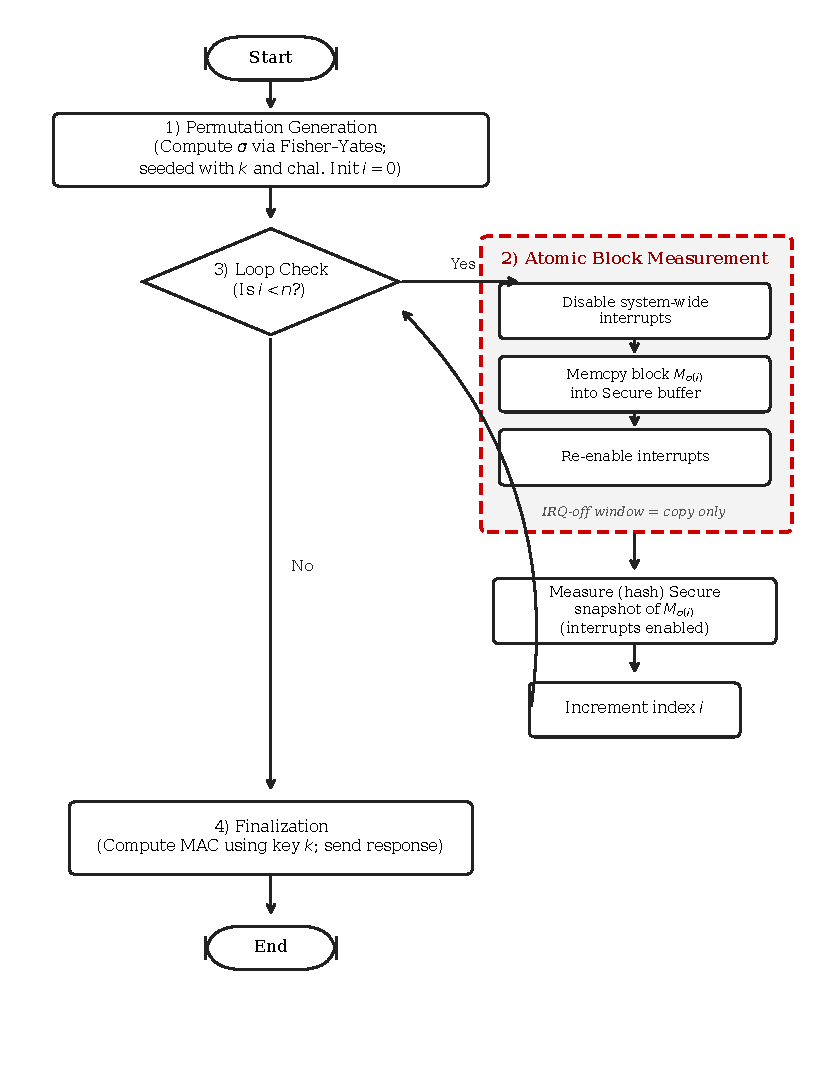
\includegraphics[width=0.92\linewidth]{atomic_workflow.pdf}
  \caption{Atomic Copy flowchart. The dashed region is the short
    interrupt-disabled window (copy only); hashing runs afterward with
    interrupts enabled.}
  \label{fig:atomic_copy_workflow}
\end{figure}

\begin{algorithm}[!ht]
\caption{Atomic Copy Secure Service}
\label{alg:atomic_copy}
\begin{algorithmic}[1]
\Require $n$ blocks, shuffled indices $\sigma$, memory $M$, key $k$
\State \Call{HMAC.Init}{$k$}
\For{$i \gets 0$ to $n-1$}
  \State $\mathit{blk} \gets M[\sigma(i)\cdot B]$
  \State \Call{DisableInterrupts}{}
  \State \Call{Memcpy}{\textit{buf}, \textit{blk}, $B$} \Comment{atomic snapshot}
  \State \Call{EnableInterrupts}{}
  \State \Call{HMAC.Update}{\textit{buf}, $B$} \Comment{interrupts on}
\EndFor
\State \textbf{return} \Call{HMAC.Finalize}{}
\end{algorithmic}
\end{algorithm}

\textbf{Security sketch.} The IRQ-off window covers only the copy, so
the snapshot that feeds HMAC is not half-updated~(S1). Key $k$ and
permutation $\sigma$ remain in Secure RAM~(S2)--(S3); hashing after the
copy uses only Secure buffer contents. We summarize preservation of
(S1)--(S3) for both designs in Section~\ref{sec:security_summary}.

\subsection{SAU Remapping}
\label{sec:sau}

Atomic Copy costs an extra Secure buffer of size $B$. SAU remapping
avoids that buffer. TrustZone-M's SAU assigns security attributes to
address ranges~\cite{armv8m-arm,an5347}. An enabled SAU region is either
Non-Secure or Secure/Non-Secure Callable; ordinary Secure memory is the
\emph{default} for addresses not covered by any enabled region. We
therefore protect each shuffled block by temporarily leaving a hole in
the Non-Secure coverage of a dedicated data window, hashing the block in
place with interrupts enabled, then restoring full-window Non-Secure
coverage (Fig.~\ref{fig:sau_memory_map}, Fig.~\ref{fig:sau_workflow},
Algorithm~\ref{alg:sau}).
Fig.~\ref{fig:sau_workflow} mirrors the Atomic Copy flowchart, but the
dashed region is a \emph{SAU-protected} window rather than an IRQ-off
copy: open a hole around $M_{\sigma(i)}$, hash in place with interrupts
enabled, then restore Non-Secure coverage.

\begin{figure}[!t]
  \centering
  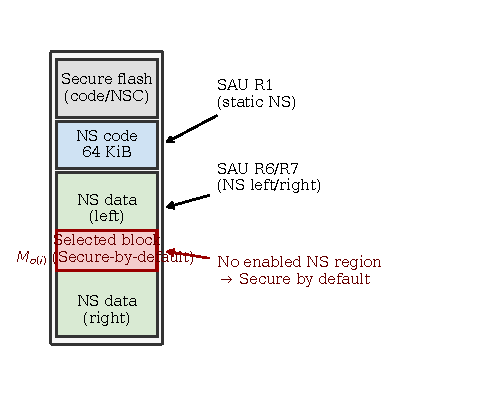
\includegraphics[width=\linewidth]{sau_memory_map.pdf}
  \caption{temporary  SAU hole over a dedicated Non-Secure data window.
    SAU region~1 covers Non-Secure code. Regions~6/7 cover the data
    surrounding the selected block; the uncovered block is Secure by
    default.\oak{"Hole" is a weird word to say here}}
  \label{fig:sau_memory_map}
\end{figure}

\begin{figure}[!t]
  \centering
  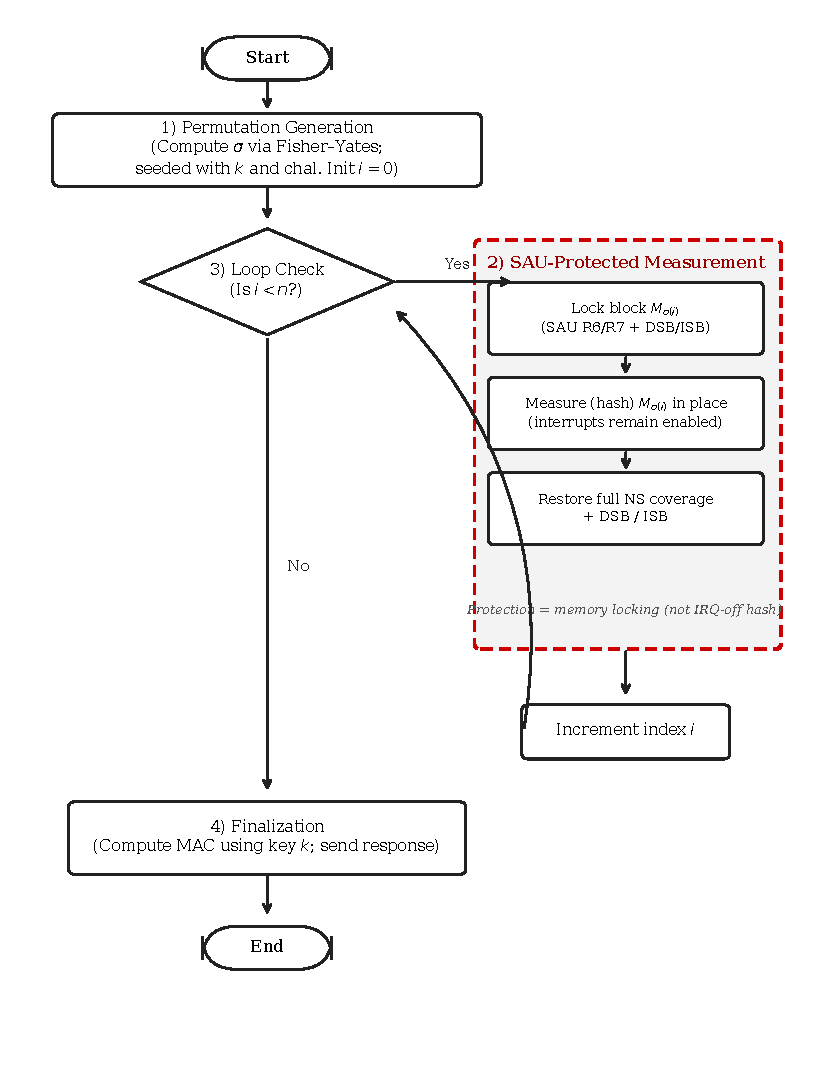
\includegraphics[width=0.92\linewidth]{sau_workflow.pdf}
  \caption{SAU hole-remapping flowchart. The dashed region protects each
    shuffled block by a temporary  Secure hole (open $\rightarrow$ hash in
    place $\rightarrow$ restore). Unlike Atomic Copy, interrupts stay
    enabled throughout; integrity comes from SAU attribution, not an
    IRQ-off copy.}
  \label{fig:sau_workflow}
\end{figure}

\begin{algorithm}[!ht]
\caption{SAU Hole-Remapping Secure Service}
\label{alg:sau}
\begin{algorithmic}[1]
\Require $n$ blocks, shuffled indices $\sigma$, data window $M$, key $k$
\State \Call{HMAC.Init}{$k$}
\State \Call{SAU.CoverWindowNS}{$M$} \Comment{rest state: window is NS}
\For{$i \gets 0$ to $n-1$}
  \State $\mathit{blk} \gets M[\sigma(i)\cdot B]$
  \State \Call{SAU.OpenHole}{\textit{blk}, $B$} \Comment{left/right NS fragments}
  \State \Call{DSB}{}; \Call{ISB}{} \Comment{block becomes Secure by default}
  \State \Call{HMAC.Update}{\textit{blk}, $B$} \Comment{in place; interrupts on}
  \State \Call{SAU.CoverWindowNS}{$M$} \Comment{restore full NS coverage}
  \State \Call{DSB}{}; \Call{ISB}{}
\EndFor
\State \textbf{return} \Call{HMAC.Finalize}{}
\end{algorithmic}
\end{algorithm}

The DSB/ISB barriers make each attribution change visible before the
next step. Non-Secure code cannot lawfully access the uncovered block
while it is Secure, whereas unrelated Non-Secure code and interrupts
remain executable~\cite{armv8m-arm}.

\textbf{Security sketch.} Opening a temporary  hole makes the selected
block Secure by default, so Non-Secure software cannot lawfully read or
write it during hashing~(S1 capture integrity without IRQ-off). Key $k$
and permutation $\sigma$ remain in Secure RAM~(S2)--(S3).
Section~\ref{sec:security_summary} summarizes both designs.
We keep the discussion at CPU SAU attribution; bus-master/DMA cases and
post-boot SAU locking used in some TF-M
platforms~\cite{tfm-isolation,tfm2024} are left to the extended version.
The attested window is placed in Non-Secure flash \emph{outside} the
application code/vector region so hole remapping never covers executable
Non-Secure pages.

\subsection{Security Properties Preserved}
\label{sec:security_summary}

Atomic Copy and SAU remapping change \emph{how} each block is captured
for hashing; they do not change SMARM's cryptographic protocol or the
placement of secrets. Both designs therefore preserve
(S1)--(S3):
\begin{itemize}
  \item \textbf{(S1) Controlled Execution.}
    Attestation still runs only through Secure/NSC entry points.
    Between blocks, interrupts remain enabled as in SMARM.
    Within a block, Atomic Copy keeps interrupts disabled for the
    entire \texttt{Memcpy}, and SAU remapping instead denies
    Non-Secure access to the uncovered block for the duration of the
    hole. In either case, untrusted software cannot splice into a
    half-captured measurement.
  \item \textbf{(S2) Key Secrecy.}
    The HMAC key $k$ never leaves Secure RAM; neither design exposes
    $k$ to Non-Secure code or to the attested data window.
  \item \textbf{(S3) Private Measurement Order.}
    The permutation $\sigma$ is derived and stored in Secure world and
    is never written to Non-Secure memory. Malware therefore still
    cannot learn the remaining visit order.
\end{itemize}
In short, Atomic Copy and SAU remapping reduce the real-time cost of
block capture while retaining SMARM's controlled execution and the
secrecy of $k$ and $\sigma$.

% ================================================================
\section{Evaluation}
\label{sec:eval}

\subsection{Setup}

All results use STM32L552ZE at $110$~MHz with FreeRTOS.
Block sizes are $B\in\{64,128,256,512,1024,2048,4096\}$~bytes.
For Atomic Copy and baseline SMARM, attested memory size is $512$~KB.
For SAU remapping we reserve a $192$~KB Non-Secure flash data window
($0\mathrm{x}08050000$--$0\mathrm{x}0807FFFF$) separate from a
$64$~KB Non-Secure code region, so hole remapping never covers
application vectors or text; FAR is measured under $1000$, $100$, and
$10$~Hz real-time tasks.
We report: (i)~TIM2-based \tdis for baseline and Atomic Copy and
(ii)~\FAR under those workloads. We omit end-to-end runtime because the
SAU prototype uses a smaller, separately reserved memory window; such a
comparison would conflate algorithmic overhead with measured size.

\subsection{Non-Interruptibility Cost}

Table~\ref{tab:tdisabled} recalls Atomic Copy versus baseline SMARM.
Atomic Copy reduces \tdis by about $15$--$16\times$ for
$B\geq 128$~bytes. SAU hole remapping removes the hash from the
interrupt-disabled path entirely: the selected block remains protected
by its Secure attribution while the hash is interruptible.

\begin{table}[!t]
  \centering
  \small
  \caption{$t_{\mathrm{disabled}}$: SMARM baseline vs.\ Atomic Copy
    (TIM2, FreeRTOS). Std.\ $<0.003$~ms.}
  \label{tab:tdisabled}
  \setlength{\tabcolsep}{3.5pt}
  \begin{tabular}{rrrrr}
    \toprule
    & \multicolumn{2}{c}{\textbf{Baseline}}
    & \multicolumn{2}{c}{\textbf{Atomic Copy}} \\
    \cmidrule(lr){2-3}\cmidrule(lr){4-5}
    \textbf{$B$} & Mean (ms) & Std & Mean (ms) & Std \\
    \midrule
    64   & 0.062 & 0.001 & $<$0.007$^\dagger$ & --- \\
    128  & 0.120 & 0.001 & 0.008 & 0.001 \\
    256  & 0.237 & 0.001 & 0.015 & 0.001 \\
    512  & 0.472 & 0.002 & 0.031 & 0.001 \\
    1024 & 0.939 & 0.001 & 0.060 & 0.001 \\
    2048 & 1.877 & 0.003 & 0.119 & 0.003 \\
    4096 & 3.749 & 0.002 & 0.243 & 0.001 \\
    \bottomrule
  \end{tabular}

  \smallskip
  \raggedright\footnotesize
  $^\dagger$Completes within one TIM2 tick ($7.27\,\mu$s).
\end{table}

\subsection{Real-Time Availability}

Figure~\ref{fig:far_three} summarizes FAR at $1000$~Hz. Baseline SMARM
degrades for large $B$, whereas Atomic Copy and corrected SAU hole
remapping remain at $\mathrm{FAR}\approx 1.0$ through
$B{=}4096$~bytes. Figure~\ref{fig:far_sau_all} reports the complete SAU
sweep: FAR remained approximately $1.0$ for all $7$ block sizes at
$10$, $100$, and $1000$~Hz ($21$ configurations).

\begin{figure}[!t]
  \centering
  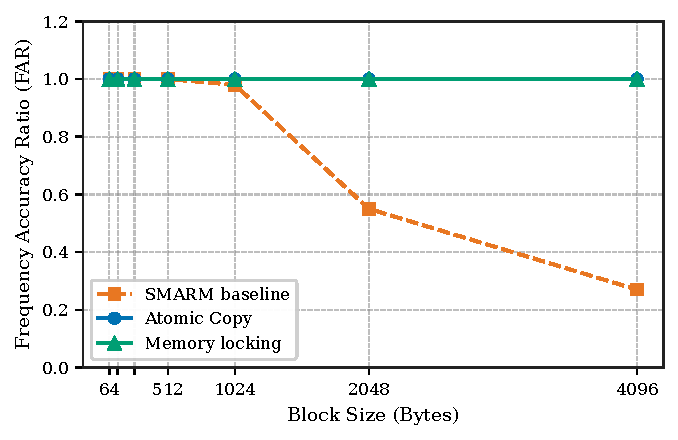
\includegraphics[width=\linewidth]{far_three_1000hz.pdf}
  \caption{FAR under a $1000$~Hz workload. Baseline SMARM loses
    activations for large blocks, whereas Atomic Copy and SAU hole
    remapping maintain FAR~$\approx 1.0$.}
  \label{fig:far_three}
\end{figure}

\begin{figure}[!t]
  \centering
  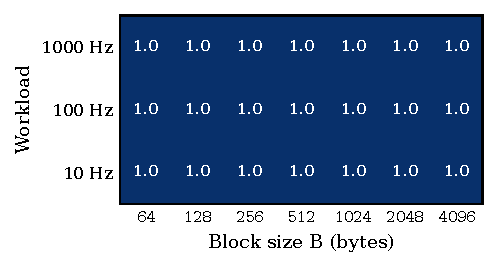
\includegraphics[width=\linewidth]{far_sau_heatmap.pdf}
  \caption{Corrected SAU hole remapping maintains FAR~$\approx 1.0$ in
    all $21$ tested block-size/workload configurations
    ($B\in\{64,\ldots,4096\}$ and $10$/$100$/$1000$~Hz).}
  \label{fig:far_sau_all}
\end{figure}

\subsection{Storage Overhead}

Atomic Copy needs one Secure buffer of size $B$ (up to $4$~KB at
$B{=}4096$). SAU remapping needs no extra measurement buffer. Both keep
$k$ and $\sigma$ in Secure RAM as in baseline SMARM.
Table~\ref{tab:storage} summarizes the trade-off: Atomic Copy pays a
small, predictable Secure RAM cost; SAU remapping avoids that buffer but
requires a dedicated Non-Secure data window that is disjoint from
application code so hole remapping never covers executable pages.

\begin{table}[!t]
  \centering
  \small
  \caption{Storage and layout overhead of the two enhancements.}
  \label{tab:storage}
  \setlength{\tabcolsep}{3.5pt}
  \begin{tabular}{lcc}
    \toprule
    \textbf{Item} & \textbf{Atomic Copy} & \textbf{SAU remapping} \\
    \midrule
    Secure copy buffer & $+B$ (up to $4$~KB) & none \\
    Extra Secure secrets & $k$, $\sigma$ & $k$, $\sigma$ \\
    Dedicated attested window & not required & $192$~KB (NS flash) \\
    Dynamic SAU regions & none & regions~6/7 \\
    \bottomrule
  \end{tabular}
\end{table}

\subsection{Summary and Design Guidance}
\label{sec:guidance}

Table~\ref{tab:metric_summary} compresses the evaluation into three axes.
Baseline SMARM fails FAR for large $B$ because hashing remains
interrupt-disabled. Both enhancements restore FAR~$\approx 1.0$, but they
pay different costs: Atomic Copy shortens the IRQ-off window to a copy
and consumes Secure RAM of size $B$; SAU hole remapping avoids that
buffer and does not disable interrupts for the hash, at the price of a
reserved Non-Secure data window and short Secure-world SAU updates.

\begin{table}[!t]
  \centering
  \small
  \caption{Summary of the three SMARM variants on FreeRTOS/TrustZone-M.}
  \label{tab:metric_summary}
  \setlength{\tabcolsep}{2.8pt}
  \renewcommand{\arraystretch}{1.15}
  \begin{tabular}{lp{0.22\linewidth}p{0.22\linewidth}p{0.28\linewidth}}
    \toprule
    & \textbf{FAR} & \textbf{IRQ-off window} & \textbf{Secure RAM / layout} \\
    \midrule
    SMARM baseline &
      Poor for large $B$ &
      Long (per-block hash) &
      No $+B$ buffer \\
    Atomic Copy &
      $\approx 1.0$ &
      Short (per-block copy) &
      $+B$ Secure buffer \\
    SAU remapping &
      $\approx 1.0$ &
      No IRQ-off for hash &
      No $+B$; reserved NS data window \\
    \bottomrule
  \end{tabular}
\end{table}

\textbf{When to prefer each enhancement.}
Platform guidance typically configures SAU once at boot as part of the
static Secure/Non-Secure map~\cite{armv8m-arm,an5347,cmsis-tz,tfm-isolation},
and production TF-M-style images often lock SAU/GTZC after that
setup~\cite{um2851,tfm2024}. Our SAU hole is therefore not a replacement
for that static partition: it is a short, Secure-only remapping of a
dedicated data window during attestation. Choose as follows:

\begin{itemize}
  \item \textbf{Atomic Copy} when Secure RAM of size $B$ is available,
    when SAU must remain locked after boot, when free SAU regions are
    scarce, or when the attested image cannot be isolated from Non-Secure
    code/vectors.
  \item \textbf{SAU remapping} when Secure RAM is tight, a dedicated
    Non-Secure data window can be reserved, and Secure software is
    allowed to reprogram SAU briefly. Because SAU/IDAU govern CPU
    attribution only, DMA or other bus masters still need platform
    controls such as GTZC~\cite{an5347}.
\end{itemize}
The conference prototype leaves SAU unlocked so the hole can be opened
and closed; locking policy and DMA-aware enforcement are left to the
extended version.

% ================================================================
\section{Related Work}
\label{sec:related}

\textbf{Classical and shuffled RA.}
SMART~\cite{eldefrawy2012smart}, VRASED~\cite{nunes2019vrased}, and
HYDRA~\cite{eldefrawy2017hydra} use long atomic measurements.
SMARM~\cite{carpent2018smarm}, PRoM~\cite{aman2021prom}, and
HAtt~\cite{aman2018hatt} use shuffled measurement to resist roving
malware while allowing interrupts between blocks. SMARM's original
prototype targeted a seL4/HYDRA stack rather than commodity RTOSes; our
baseline is a FreeRTOS/TrustZone-M port of that protocol, against which
we evaluate the two enhancements above.

\textbf{Interruptible attestation.}
ISC-FLAT~\cite{isc-flat}, ASAP~\cite{asap}, and IDA~\cite{ida2024}
handle interrupts in control-flow or hybrid attestation. They are
complementary; we target memory-content RA under FreeRTOS.

\textbf{TrustZone-M and SAU.}
TrustZone-M and SAU define CPU security
attribution~\cite{trustzone2025,armv8m-arm,an5347,cmsis-tz}. TF-M and
vendor TFM examples usually set a static SAU map early and may lock it
until reset~\cite{tfm2024,tfm-isolation,um2851}. We instead use a short
dynamic SAU hole as an alternative to copying a block into Secure RAM
during SMARM measurement, and discuss when that choice is appropriate
in Section~\ref{sec:guidance}.

\textbf{Custom hardware.}
LO-FAT~\cite{lo-fat}, LiteHAX~\cite{litehax}, and ATRIUM~\cite{atrium}
remove non-interruptible windows with dedicated hardware. We stay on
unmodified TrustZone-M MCUs.

% ================================================================
\section{Conclusion}
\label{sec:conclusion}

SMARM improves RA interactivity, but interrupt-disabled hashing still
hurts FAR for large blocks on FreeRTOS/TrustZone-M. Atomic Copy cuts
that window to a memory copy and restores FAR~$\approx 1.0$ with a
buffer of size $B$. SAU hole remapping achieves similar FAR without a
copy buffer and keeps FAR~$\approx 1.0$ across all tested block sizes
and $10$--$1000$~Hz workloads. Both enhancements preserve SMARM's
security properties~(S1)--(S3): controlled Secure/NSC entry with
integrity of each block capture, secrecy of $k$, and privacy of the
measurement order~$\sigma$. In practice, prefer Atomic Copy when
Secure RAM is available or SAU must stay locked, and prefer SAU
remapping when a dedicated data window can absorb temporary  attribution
changes without an extra Secure buffer.

\bibliographystyle{IEEEtran}
\bibliography{citation}

\end{document}
